\documentclass[letterpaper, 12pt]{article}

\usepackage{geometry}
 \geometry{
 letterpaper,
 total={170mm,257mm},
 left=20mm,
 top=20mm,
 bottom=20mm
 }
\usepackage{graphicx} % Required for inserting images
\usepackage{authblk}
\usepackage{amssymb}
\usepackage{lipsum}
\usepackage{float}
\usepackage{times}
\usepackage{amsmath}
\usepackage[format=plain,
            labelfont={bf,it},
            textfont=it]{caption}
\captionsetup{justification=raggedright,singlelinecheck=false}
\usepackage{ragged2e}
\usepackage{longtable}
\usepackage{comment}
\usepackage{setspace}
\usepackage{fancyhdr}
\usepackage{titlesec}
\usepackage[hyperindex,breaklinks]{hyperref}
\hypersetup{
    colorlinks=true,
    linkcolor=blue,
    filecolor=magenta,      
    urlcolor=blue
    }
% \usepackage{background} % add COSIG logo to page
\usepackage[T1]{fontenc}
\usepackage{helvet}
\renewcommand{\familydefault}{\sfdefault}
\pagenumbering{gobble}
\usepackage[skip=10pt plus1pt, indent=40pt]{parskip}

\titlespacing*{\section}
{0pt}{1.5ex plus 1ex minus .2ex}{1.3ex plus .2ex}

\renewcommand\Authfont{\fontsize{12}{14.4}\selectfont}
\renewcommand\Affilfont{\fontsize{9}{10.8}\itshape}
 
\begin{document}
\flushleft

\includegraphics[width=0.5\textwidth]{img/home/241017_final_logo_mockup.png}

\section*{Suspicious venues}
\addcontentsline{toc}{section}{Suspicious venues}
\textit{Last updated: 4 May 2025}

Problematic papers repeatedly showing up in the same publication venue (e.g., journal, conference, book, etc.) can raise warning signs about the venue itself. A well-structured and thorough peer review system at such venues is unlikely to result in frequent publication of glaringly problematic articles.

When such venues are implicated or exhibit red flags on their own, it can indicate that the papers they published deserve additional scrutiny.
This does not always indicate the publisher itself is malicious, as many publishers do not closely scrutinize the papers they publish.
Thus, legitimate world-renowned venues can share a publisher with shady venues that publish obvious nonsense (see problematic articles published in \href{https://solalpirelli.github.io/2023/01/25/troubling-acm-venues.html}{Association for Computing Machinery conferences} and \href{https://deevybee.blogspot.com/2025/02/ieee-has-pseudoscience-problem.html}{Institute of Electrical and Electronics Engineers conferences}).

This guide covers common warning signs that a publication venue deserves additional scrutiny. Many additional warning signs are described by \href{https://doi.org/10.1177/0192623320920209}{Elmore et al. (2020)}.

\subsection*{Missing or outdated information}

The organizers of unethical venues are not interested in spending any more time than is necessary.
This often results in venue websites that are not up to date or outright broken outside of the main page.

Would a reasonable person easily find the information they need to gauge their interest,
write a paper with the right specifications, and submit that paper?
For a conference, would this reasonable person also easily know when and where the conference is held and how to get there?

Missing information, copy-pasted text from previous years that contains outdated dates and times,
and ``404 Not Found'' pages are all red flags.
Sometimes the information looks real, but a quick check will reveal it is not,
such as international conferences supposedly taking place in buildings that are
obviously not suitable for a large number of attendees nor for presentations or \href{https://doi.org/10.1038/d41586-024-02358-w}{multiple conferences taking place in the same location on the same day}.

\subsection*{Overemphasis on metrics}

Scientists and insitutions around the globe are often evaluated using quantitative heuristics such as number of articles published in indexed journals and number of citations to those articles (see \href{https://osf.io/zpf4r}{COSIG's citations guide}). Unethical and predatory venues often emphasize common metrics well beyond how a reasonable venue would.

Unethical venues may include in their description the fact they are Scopus-indexed,
the fact that proceedings will be published with a specific well-known publisher (without providing any additional details)
and other information that should be obvious and unstated for any reputable venue.
If a venue tries too hard to convince you that it is legitimate, it likely is not.

\subsection*{Malicious compliance with integrity standards}

To be attractive in terms of metrics such as indexing in a particular database,
unethical venues often abuse the trust of a reputable publisher.
Reputable publishers try to maintain their reputation with basic integrity standards, such as the absence of plagiarism (see \href{https://osf.io/ntcb4}{COSIG's plagiarism guide}).

Unethical venues work around this by turning subjective checks into objective ones
and giving enough information to authors to avoid detection.
For instance, submissions to a venue will often be assessed by a human with the help of a tool such as
\href{https://www.ithenticate.com/}{iThenticate}.
To work around this, a malicious editor-in-chief can publicly state which tool will be used
and which exact threshold will be used on the tool output to make a binary assessment of plagiarism.
Thus, authors wishing to plagiarize only need to spend as little time as necessary hiding their plagiarism
until the tool's output is below the threshold.
Any ``plagiarism score'' threshold indicates a problematic venue.

\subsection*{Unrealistic review time}

Sending papers for peer review, receiving the reviews, and coming to a decision takes time.
Turnaround times can be shorter for venues that have specific deadlines, such as conferences,
since finding the reviewers is already done and these reviewers know to block time in their calendar.
However, peer review time is still normally measured in months. There is also no guarantee that a submission that goes out to peer review will actually be accepted.

Any venue that advertises a guaranteed time to acceptance should be regarded with extreme suspicion. Any venue that advertises an extremely short review period (unless submissions are very short, e.g., only abstracts) are likely predatory or otherwise fraudulent.

Journals will often list the time between submission and acceptance, allowing for estimation of times to publication. Suspicious venues will often routinely accept papers from particular authors in a matter of days, not nearly long enough for legitimate peer review to occur.
which often state when they were submitted and accepted.
This can reveal unethical patterns where papers from some authors are supposedly reviewed in days.
(\href{https://deevybee.blogspot.com/2015/02/editors-behaving-badly.html}{example})

Note that not all journals provide accurate submission information. Sometimes, the listed ``submission'' date is really a resubmission after revisions were requested by reviewers.

\subsection*{Unethical editors}

Unethical venues can often be spotted by suspicious behavior by their editors.

While it is normal for well-known scientists to chair well-known venues while also publishing in them,
some editors do not stop at the low number of papers one would expect from a reputable scientist,
and instead \href{https://deevybee.blogspot.com/2020/08/pepiops-prolific-editors-who-publish-in.html}{publish dozens of papers in their own venue}, abusing their position of power.

Venues that publish articles wherein \href{https://pubpeer.com/publications/57BB3F8859A0F5BE6FBC4DB70F2E8E}{an outsize portion of an article's citations are to the venue's editor(s)} should be regarded with extreme suspicion. Citing multiple papers from the editor of the venue
can be acceptable if that person has published foundational work,
but many articles in a venue all citing the exact same set of papers from the editors is unexpected.

\subsection*{Fake committees}

Unethical venues will often project legitimacy by listing legitimate scientists' names as conference organizers, editors or peer reviewers without their knowledge or consent. These venues might fabricate affiliations or contact information alongside the names of real scientists or might use real scientists' pictures to represent fictitious identities. 

If you suspect reviewer names are being used without their knowledge, find the contact information for the reviewers
using a source unrelated to the venue under suspicion and contact them. Most institutions provide some form of public profile for researchers,
even if it is merely a directory entry with just a name.
If you suspect a reviewer identity or affiliation has been fabricated, find a contact at the provided affiliation and ask.

\subsection*{Hijacked journals}

Often illegitimate publishers will `hijack' existing legitimate journals by creating a website that mimics that of the existing journal, using the existing journal's name and/or \href{https://portal.issn.org/}{International Standard Serial Number}, or registering the existing journal's domain after it has expired. Having hijacked the existing journal's brand, the illegitimate publisher can now publish whatever content it pleases while enjoying the benefits of the journal's existing reputation (including membership in curated literature databases, see `Indexing and de-indexing' below).

The \href{https://retractionwatch.com/the-retraction-watch-hijacked-journal-checker/}{Retraction Watch Hijacked Journal Checker} is an updating directory of journals that have been hijacked.

\pagebreak

\begin{figure}[h!tbp]
    \centering
    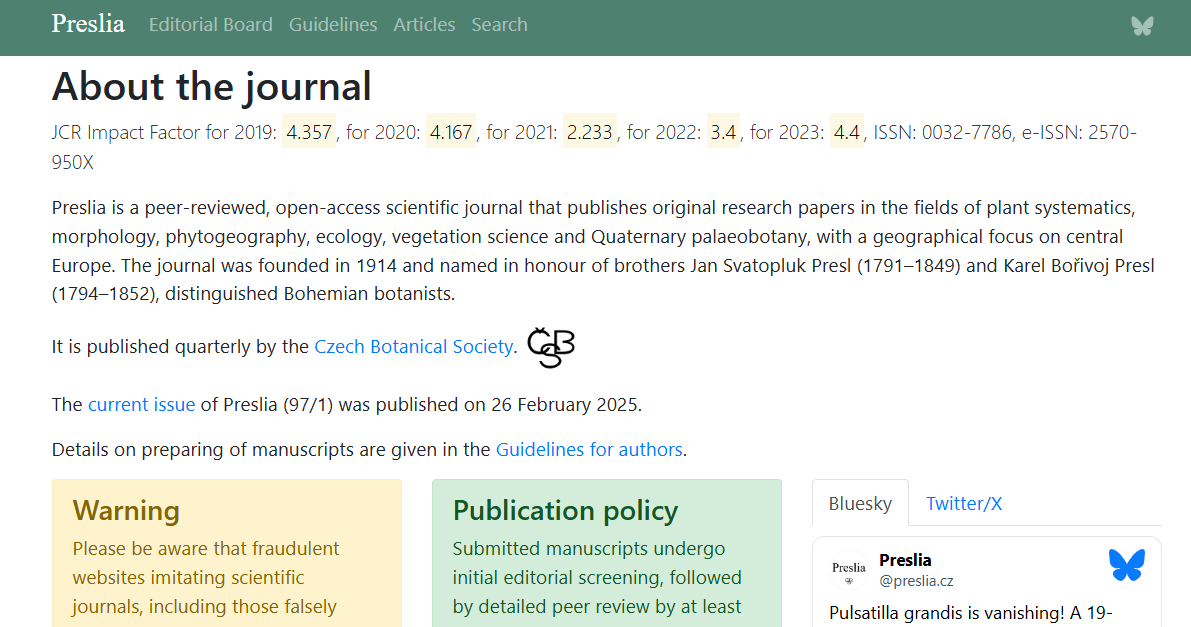
\includegraphics[width=\textwidth]{img/venues/Preslia original.png}
    \caption*{The homepage of the legitimate journal Preslia, a publication of the Czech Botanical Society, at \href{https://www.preslia.cz}{www.preslia.cz}.}
\end{figure}

\begin{figure}[h!tbp]
    \centering
    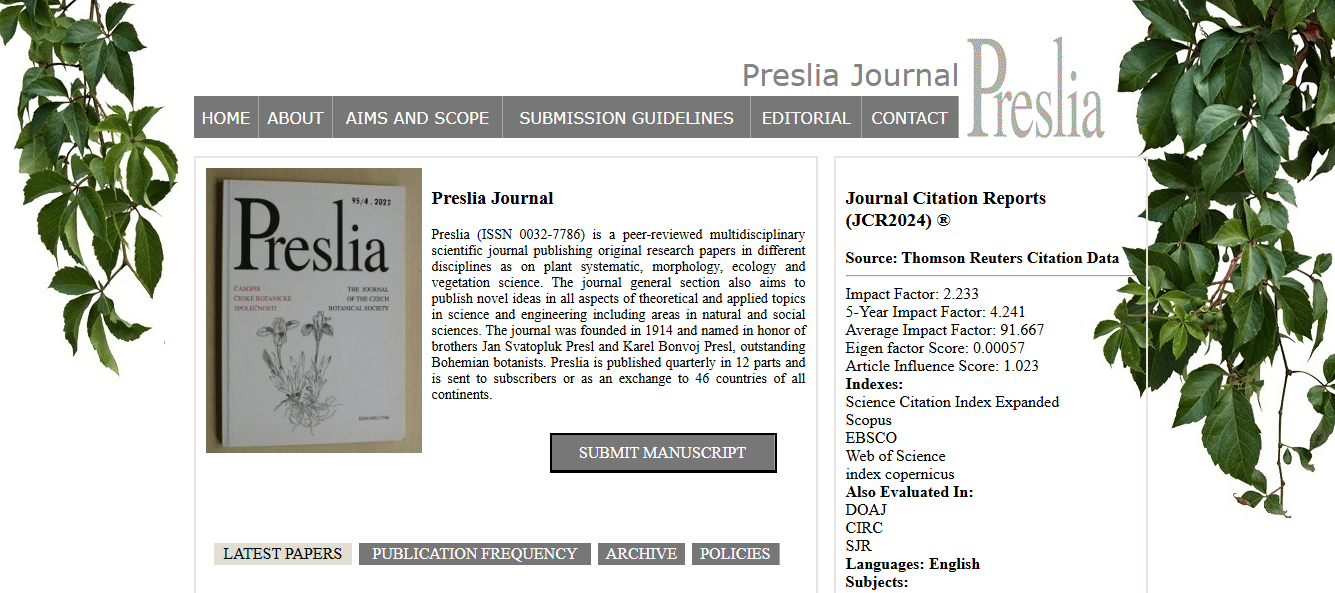
\includegraphics[width=\textwidth]{img/venues/Preslia hijacked-min.png}
    \caption*{The homepage of a hijacked version of Preslia at \href{https://presliajournal.com/}{www.presliajournal.com}. Note that the hijacked journal appropriates Preslia's ISSN and claims to accept papers on any topic, despite the actual Preslia being solely a botany journal.}
\end{figure}

\subsection*{Raising suspicions about a venue on PubPeer}

To report concerning trends in a venue's articles, you can write a lengthy PubPeer comment on one paper
and short comments on the others linking to the main comment (see \href{https://osf.io/sghaq}{COSIG's guide on PubPeer commenting}).
Alternatively, if there is a DOI representing the totality of articles in a venue (e.g., front matter for a conference or an article listing journal editorial board members), considering writing a \href{https://pubpeer.com/search?q=\%22proceedings-level+report\%22}{``proceedings-level report''} or \href{https://pubpeer.com/search?q=\%22journal-level+report\%22}{``journal-level report''}.

\subsection*{Indexing and de-indexing}

Publication venues are `indexed' by literature aggregators like \href{https://www.webofscience.com/wos/}{Web of Science}, \href{https://www.scopus.com}{Scopus} and \href{https://www.nlm.nih.gov/medline/medline_home.html}{MEDLINE} and in databases like the \href{https://doaj.org/}{Directory of Open Access Journals (DOAJ)}. Being indexed by one of these services is perceived as a marker of quality for publication venues. Many predatory venues advertise their indexing status because they know that many academics are required to publish papers only in indexed venues. These services will sometimes withdraw the indexing status of , or `de-index', particular venues because of a pattern of publication integrity issues or other ethical violations (for example, see the \href{https://docs.google.com/spreadsheets/d/1Kv3MbgFSgtSDnEGkA2JacrSjunRu0umHeZCtcMeqO5E/edit?gid=2104690845\#gid=2104690845}{list of journals withdrawn from DOAJ}, many of which have been removed for ``not adhering to Best Practice''). If you have suspicions about a venue and it is indexed by one of these services, consider reporting your concerns to the service.

\subsection*{Additional resources}

\begin{itemize}
    \setlength\itemsep{-0.5em}
    \item \href{https://doi.org/10.1177/0192623320920209}{``Predatory Journals: What They Are and How to Avoid Them'' (2020)}
    \item \href{https://retractionwatch.com/2024/10/01/hidden-hydras-uncovering-the-massive-footprint-of-one-paper-mills-operations/}{``Hidden hydras: uncovering the massive footprint of one paper mill’s operations'' (2024)}
    \item \href{https://deevybee.blogspot.com/2015/02/editors-behaving-badly.html}{``Editors behaving badly?'' (2015)}
    \item \href{https://deevybee.blogspot.com/2024/09/using-pubpeer-to-screen-editors.html}{``Using PubPeer to screen editors'' (2024)}
    \item \href{https://deevybee.blogspot.com/2020/08/pepiops-prolific-editors-who-publish-in.html}{``PEPIOPs – prolific editors who publish in their own publications'' (2020)}
    \item \href{https://www.science.org/content/article/it-felt-very-icky-scientist-s-name-was-used-write-fake-peer-reviews}{```It felt very icky': This scientist's name was used to write fake peer reviews'' (2024)}
    \item \href{https://doi.org/10.47989/irpaper912}{``Membership of the editorial boards of journals published by the predatory publisher OMICS: willing and unwilling participation'' (2021)}
    \item \href{https://doi.org/10.1038/543481a}{``Predatory journals recruit fake editor'' (2017)}
    \item \href{https://doi.org/10.18421/GP19.02-06}{``The full story of 90 hijacked journals from August 2011 to June 2015'' (2015)}
    \item \href{https://retractionwatch.com/2020/07/07/the-case-of-the-stolen-journal/}{``The case of the stolen journal'' (2020)}
    \item \href{https://doi.org/10.1007/s11192-021-04056-0}{``Detecting a network of hijacked journals by its archive'' (2021)}
    \item \href{https://doi.org/10.1002/asi.24855}{``Challenges posed by hijacked journals in Scopus'' (2023)}
    \item \href{https://doi.org/10.1080/08989621.2024.2387210}{``Prevalence of plagiarism in hijacked journals: A text similarity analysis'' (2024)}
    \item \href{https://doi.org/10.1126/science.zcgp0a2}{``Leading scholarly database listed hundreds of papers from ‘hijacked’ journals'' (2023)}
    \item \href{https://retractionwatch.com/the-retraction-watch-hijacked-journal-checker/}{The Retraction Watch Hijacked Journal Checker}
\end{itemize}

\end{document}